%!TEX encoding = UTF-8 Unicode
\documentclass{lecturenotes}

\renewcommand{\vecka}{6}
\newcommand{\veckotema}{Klasser}

%!TEX encoding = UTF-8 Unicode
\setbeamertemplate{footline}[frame number]

\newcommand{\LibVersion}{0.1.0} % latest version of introlib at https://github.com/lunduniversity/introprog-scalalib
\newcommand{\LibJar}{\texttt{introprog-\LibVersion.jar}}
\newcommand{\JDKApiUrl}{\url{https://docs.oracle.com/javase/8/docs/api/}}


\title[Föreläsningsanteckningar EDAA45, \CurrentYear]{EDAA45 Programmering, grundkurs}
\subtitle{Läsvecka \vecka: \veckotema}
\author{Björn Regnell}
\institute{Datavetenskap, LTH}
\date{Lp1-2, HT \CurrentYear}

%!TEX encoding = UTF-8 Unicode

\newcommand{\ModWeekONE}{Introduktion}
\newcommand{\ExeWeekONE}{expressions}
\newcommand{\LabWeekONE}{kojo}


\newcommand{\ModWeekTWO}{Program, kontrollstrukturer}
\newcommand{\ExeWeekTWO}{programs}
\newcommand{\LabWeekTWO}{--}


\newcommand{\ModWeekTHREE}{Funktioner, abstraktion}
\newcommand{\ExeWeekTHREE}{functions}
\newcommand{\LabWeekTHREE}{irritext}


\newcommand{\ModWeekFOUR}{Objekt, inkapsling}
\newcommand{\ExeWeekFOUR}{objects}
\newcommand{\LabWeekFOUR}{blockmole}


\newcommand{\ModWeekFIVE}{Klasser, datamodellering}
\newcommand{\ExeWeekFIVE}{classes}
\newcommand{\LabWeekFIVE}{--}


\newcommand{\ModWeekSIX}{Mönster, felhantering}
\newcommand{\ExeWeekSIX}{patterns}
\newcommand{\LabWeekSIX}{blockbattle}


\newcommand{\ModWeekSEVEN}{Sekvenser, enumerationer}
\newcommand{\ExeWeekSEVEN}{sequences}
\newcommand{\LabWeekSEVEN}{shuffle}


\newcommand{\ModWeekEIGHT}{Matriser, typparametrar}
\newcommand{\ExeWeekEIGHT}{matrices}
\newcommand{\LabWeekEIGHT}{life}


\newcommand{\ModWeekNINE}{Mängder, tabeller}
\newcommand{\ExeWeekNINE}{lookup}
\newcommand{\LabWeekNINE}{words}


\newcommand{\ModWeekTEN}{Arv, komposition}
\newcommand{\ExeWeekTEN}{inheritance}
\newcommand{\LabWeekTEN}{snake0}


\newcommand{\ModWeekELEVEN}{Kontextuella abstraktioner, api}
\newcommand{\ExeWeekELEVEN}{context}
\newcommand{\LabWeekELEVEN}{snake1}


\newcommand{\ModWeekTWELVE}{Valfri fördjupning, Projekt}
\newcommand{\ExeWeekTWELVE}{extra}
\newcommand{\LabWeekTWELVE}{Projekt0}


\newcommand{\ModWeekTHIRTEEN}{Repetition}
\newcommand{\ExeWeekTHIRTEEN}{examprep}
\newcommand{\LabWeekTHIRTEEN}{Projekt1}


\newcommand{\ModWeekFOURTEEN}{Muntligt prov}
\newcommand{\ExeWeekFOURTEEN}{Munta}
\newcommand{\LabWeekFOURTEEN}{Munta}


 
\begin{document}

\frame{\titlepage}
\setnextsection{\vecka}
\section[Vecka \vecka: \veckotema]{\veckotema}
\frame{\tableofcontents}

%!TEX encoding = UTF-8 Unicode
%!TEX root = ../lect-week06.tex

%%%

\Subsection{Vad är en klass?}

\begin{Slide}{Vad är en klass?}
\begin{itemize} 
\item En klass är en mall för att skapa objekt. 
\item Objekt skapas med \code{new Klassnamn} och kallas för  \Emph{instanser} av klassen \code{Klassnamn}.
\item En klass innehåller medlemmar \Eng{members}: 
  \begin{itemize} 
  \item \Emph{attribut}, kallas även fält \Eng{field}: \code{val}, \code{lazy val}, \code{var} 
  \item \Emph{metoder}, kallas även operationer: \code{def}
  \end{itemize}
\item Varje instans har sin uppsättning värden på attributen (fälten).
\end{itemize}

\end{Slide}


\ifkompendium\else


\begin{Slide}{Vad är en klass?}\SlideFontSmall
Metafor: En klass liknar en \Emph{stämpel}
\begin{figure}
\centering
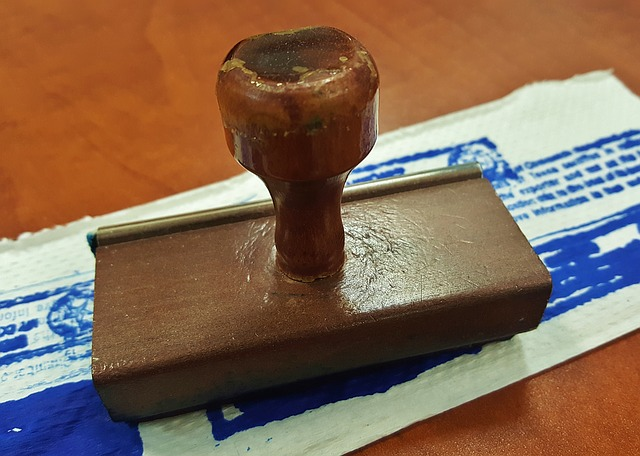
\includegraphics[width=0.5\textwidth]{../img/stamp}
\end{figure}
\begin{itemize}
\item En stämpel kan tillverkas -- motsvarar deklaration av klassen. 
 \item Det händer inget förrän man stämplar -- motsvarar \code{new}.
\item Då skapas avbildningar -- motsvarar instanser av klassen.


\end{itemize}
\end{Slide}


\begin{Slide}{Klassdeklarationer och instansiering}\SlideFontSmall
\setlength{\leftmargini}{0pt}
\begin{itemize}
\item Syntax för deklaration av klass: \\ \vspace{0.5em}{\SlideFontSize{13}{16}\code|class Klassnamn(parametrar){ medlemmar }|}\vspace{0.5em}



\item Exempel \Emph{deklaration}:
\begin{Code}
class Klassnamn(val attribut1: Int, attribut2: String){  
  val attribut3: Double = 42.0              //publikt oföränderligt attribut
  private var attribut3: Boolean = false    //privat medlem syns inte utåt
  def metod(parameter: Int) = parameter + 1 //funktion i klass kallas metod
  lazy val attr4 = Vector.fill(100000)(42.0)     //fördröjd initialisering 
}
\end{Code}

\item Parametrar initialiseras med de argument som ges vid \code{new}. 
\item Exempel \Emph{instansiering}:
\begin{Code}
val instansReferens = new Klassnamn(42, "hej")
\end{Code}

\item Attribut blir \Emph{publika} (alltså synliga utåt) om inte modifieraren \code{private} anges.
\item Parametrar som inte föregås av modifierare (t.ex. private val, val, var) blir attribut som är: \code{ private[this] val } och bara synliga i \Alert{denna} instans.

\end{itemize}
\end{Slide}


\begin{Slide}{Exempel: Klassen Complex i Scala}\SlideFontSmall
\begin{Code}
class Complex(val re: Double, val im: Double){
  def r  = math.hypot(re, im)
  def fi = math.atan2(re, im)
  def +(other: Complex) = new Complex(re + other.re, im + other.im)
  var imSymbol = 'i'
  override def toString = s"$re + $im$imSymbol"
}
\end{Code}

\begin{REPL}
scala> val c1 = new Complex(3, 4)
c1: Complex = 3.0 + 4.0i

scala> val polarForm = (c1.r, c1.fi)
polarForm: (Double, Double) = (5.0,0.6435011087932844)

scala> val c2 = new Complex(1, 2)
c2: Complex = 1.0 + 2.0i

scala> c1 + c2
res0: Complex = 4.0 + 6.0i
\end{REPL}

%TODO:
%  \begin{itemize} 
%  \item Bygg upp \code{case class Complex(re: Double, im: Double)} steg för steg inspirerat av Pins3ed kap 6 i likhet med hur de gör med Rational
%  \item Illustrera följande begrepp: this (behövs i max(that)), method overloading behövs för att plussa med både Complex och Double
%  \item Till fördjupningsövning: dekorera Double med metoderna im och re samt (Double, Double) med metoden ir (för irrational) med implicit klass
%  \item Till extrauppgift: implementera klassen Polar(r, fi) med polära koordinater \url{https://sv.wikipedia.org/wiki/Pol%C3%A4ra_koordinater}
%  \end{itemize}
\end{Slide}

\begin{Slide}{Exempel: Principen om enhetlig access}\SlideFontSmall
\begin{Code}
class Complex(val re: Double, val im: Double){
  val r  = math.hypot(re, im)
  val fi = math.atan2(re, im)
  def +(other: Complex) = new Complex(re + other.re, im + other.im)
  var imSymbol = 'i'
  override def toString = s"$re + $im$imSymbol"
}
\end{Code}
\pause
\begin{itemize}
\item Efter som attributen \code{re} och \code{im} är oföränderliga, kan vi lika gärna ändra i klass-implementationen och göra om metoderna \code{r} och \code{fi} till \code{val}-variabler utan att klientkoden påverkas. 

\item Då anropas \code{math.hypot} och \code{math.atan2} bara en gång vid initialisering (och inte varje gång som med \code{def}).

\item Vi skulle även kunna använda \code{lazy val} och då bara räkna ut \code{r} och \code{fi} om och när de verkligen refereras av klientkoden, annars inte.

\item Eftersom klientkoden inte ser skillnad på metoder och variabler, kallas detta \Emph{principen om enhetlig access}. (Många andra språk har \Alert{inte} denna möjlighet, tex Java.)

\end{itemize}

\end{Slide}


\begin{Slide}{Exempel: Motsvarande klass JComplex i Java}\SlideFontSmall
\javainputlisting[basicstyle=\SlideFontSize{5}{6}\ttfamily\selectfont]{../compendium/examples/JComplex.java}
\end{Slide}

\begin{Slide}{Exempel: Använda JComplex från Scala}
\begin{REPL}
$ javac JComplex.java 
$ scala
Welcome to Scala 2.11.8 (Java HotSpot(TM) 64-Bit Server VM, Java 1.8.0_66).
Type in expressions for evaluation. Or try :help.

scala> val jc1 = new JComplex(3, 4)
jc1: JComplex = 3.0 + 4.0i

scala> val polarForm = (jc1.getR, jc1.getFi)
polarForm: (Double, Double) = (5.0,0.6435011087932844)

scala> val jc2 = new JComplex(1, 2)
jc2: JComplex = 1.0 + 2.0i

scala> jc1 add jc2
res0: JComplex = 4.0 + 6.0i
\end{REPL}
\end{Slide}


\begin{Slide}{Exempel: Test av JComplex i Java}
\javainputlisting[basicstyle=\SlideFontSize{9}{11}\ttfamily\selectfont]{../compendium/examples/JComplexTest.java}
\begin{itemize}
\item Tupler finns inte i Java, så det går inte på ett enkelt sätt att i Java skapa par av värden somi Scala.

\item Operatornotation för metoder finns inte i Java, så man måste i Java använda punktnotation och skriva: \code{jc1.add(jc2)}
\end{itemize}
\end{Slide}


\Subsection{Instansiering: \texttt{new}}

\begin{Slide}{Instansiering med \texttt{new}}
Rita molbild med instanser av klassen Complex
\end{Slide}

\begin{Slide}{Instansiering med fabriksmetod}
\end{Slide}

\begin{Slide}{Instansiering med default-argument}
\end{Slide}

\begin{Slide}{Instansiering med alternativa fabriksmetoder}
\end{Slide}

\begin{Slide}{Förändringsbar eller oföränderlig?}
\end{Slide}


\Subsection{Referens saknas: \texttt{null}}

\begin{Slide}{Referens saknas: \texttt{null}}
\end{Slide}


\begin{Slide}{Konstruktor}
\end{Slide}

\begin{Slide}{Skräpsamling}
Destruktor
\end{Slide}

\Subsection{Synlighet}

\begin{Slide}{Synlighet}
definiera/förklara:
private
private[this]
\end{Slide}

\begin{Slide}{Kompanjonsobjekt}
\end{Slide}


\begin{Slide}{Synlighet av klassparametrar i klasser \& case-klasser}\SlideFontSmall
\code{private[this]} är \Alert{ännu} mer privat än \code{private} 
\begin{Code}
class Hemlis(private val hemlis: Int) {
  def ärSammaSom(annan: Hemlis) = hemlis == annan.hemlis   // Funkar!
}

class Hemligare(private[this] val hemlis: Int) {
  def ärSammaSom(annan: Hemligare) = hemlis == annan.hemlis //KOMPILERINGSFEL
}
\end{Code}
Vad händer om man inte skriver något? Olika för klass och case-klass:
\begin{Code}
class Hemligare(hemlis: Int) { // motsvarar private[this] val
  def ärSammaSom(annan: Hemligare) = hemlis == annan.hemlis //KOMPILERINGSFEL
}

case class InteHemlig(seMenInteRöra: Int) { // blir automatiskt val 
  def ärSammaSom(annan: InteHemlig): Boolean = 
    seMenInteRöra == annan.seMenInteRöra 
}

\end{Code}
\end{Slide}


\Subsection{Klasser i Java}

\begin{Slide}{Klasser i Java}
\end{Slide}

\begin{Slide}{Statiska medlemmar}
\end{Slide}


\Subsection{Getters och setters}

\begin{Slide}{Getters och setters i Java}
\end{Slide}

\begin{Slide}{Getters och setters i Scala}
\end{Slide}

\begin{Slide}{Ändra attributrepresentation utan att påverka existerande kod}
Complex som polära koordinater i Java med privat attribut
Complex som polära koordinater med publika attribut om man har enhetlig access
\end{Slide}


\Subsection{Implementation saknas: ???}

\begin{Slide}{Implementation saknas: ???}
\end{Slide}


\fi


%!TEX encoding = UTF-8 Unicode
%!TEX root = ../lect-week06.tex

%%%

\ifkompendium\else

\Subsection{Likhet}
\begin{Slide}{Referenslikhet eller strukturlikhet?}\SlideFontSmall
Det finns två \Alert{principiellt olika} sorters \Emph{likhet}:
\begin{itemize}
\item \Emph{Referenslikhet} \Eng{refernce equality} där två referenser anses lika om de refererar till \Emph{samma instans} i minnet.
\item \Emph{Strukturlikhet} \Eng{structural equality} där två referenser anses lika om de refererar till instanser med \Emph{samma innehåll}.

\pause

\item I Scala finns flera metoder som testar likhet:
\begin{itemize}\SlideFontSmall
\item metoden \code{eq} testar referenslikhet och \code{r1.eq(r2)} ger \code{true} om \code{r1} och \code{r2} refererar till \Emph{samma} instans.

\item metoden \code{ne} testar referens\textbf{o}likhet och \code{r1.ne(r2)} ger \code{true} om \code{r1} och \code{r2} refererar till \Alert{olika} instanser.

\item metoden \code{==} som anropar metoden \code{equals} som default testar referenslikhet men som \Alert{kan överskuggas} om man \Emph{själv vill bestämma} om det ska vara referenslikhet eller strukturlikhet.
\end{itemize}

\pause

\item Scalas \Emph{standardbibliotek} och \Emph{grundtyperna} \code{Int}, \code{String} etc. testar \Emph{strukturlikhet} genom metoden \code{==}
\pause
\item I Java är det annorlunda: symbolen \code{==} är ingen metod i Java utan specialsyntax som  testar referenslikhet mellan instanser, medan metoden \code{equals} kan överskuggas med valfri likhetstest.
\end{itemize}
\end{Slide}


\begin{Slide}{Exempel: referenslikhet och strukturlikhet}
I Scalas standardbibliotek har man överskuggat \code{equals} så att metoden \code{==} ger test av \Emph{strukturlikhet} mellan instanser:
\begin{REPL}
scala> val v1 = Vector(1,2,3)
v1: scala.collection.immutable.Vector[Int] = Vector(1, 2, 3)

scala> val v2 = Vector(1,2,3)
v2: scala.collection.immutable.Vector[Int] = Vector(1, 2, 3)

scala> v1 eq v2                //referenslikhetstest: olika instanser
res0: Boolean = false

scala> v1 ne v2
res1: Boolean = true

scala> v1 == v2                //strukturlikhetstest: samma innehåll
res2: Boolean = true

scala> v1 != v2
res3: Boolean = false
\end{REPL}
\end{Slide}


\begin{Slide}{Referenslikhet och egna klasser}
Om du inte gör något speciellt med dina egna klasser så ger metoden \code{==} test av \Emph{referenslikhet} mellan instanser:
\begin{REPLnonum}
scala> class Gurka(val vikt: Int)

scala> val g1 = new Gurka(42)
g1: Gurka = Gurka@2cc61b3b

scala> val g2 = new Gurka(42)
g2: Gurka = Gurka@163df259

scala> g1 == g2       // samma innehåll men olika instanser
res0: Boolean = false

scala> g1. vikt == g2. vikt
res1: Boolean = true
\end{REPLnonum}
\end{Slide}

\fi


%!TEX encoding = UTF-8 Unicode
%!TEX root = ../lect-week06.tex

%%%
\ifkompendium\else


\Subsection{Case-klasser och likhet}



\begin{Slide}{Varför case-klass?}
Med case-klasser får du mycket ''godis på köpet'':
\begin{itemize}
\item Skapa \Emph{oföränderlig datastruktur} med få kodrader.
\item Klassparametrar blir automatiskt publika \code{val}-attribut (inte \texttt{private[this]} som i vanliga klasser).
\item Du får en automatisk \Emph{toString} som ger klassens namn och värdet av alla \code{val}-attribut som ges av klassparametrarna.
\item Du slipper skriva \code{new} eftersom du får ett automatiskt kompanjonsobjekt med en fabriksmetod \code{apply} för indirekt instansiering där alla klassparametrarnas \code{val}-attribut initialiseras.
\item Metoden \code{==} ger \Emph{strukturlikhet} (och inte referenslikhet).
\end{itemize}
\end{Slide}



\begin{Slide}{Likhet och case-klasser}
Metoden \code{equals} är i case-klasser automatiskt överskuggad så att metoden \code{==} ger test av strukturlikhet. 
\begin{REPL}
scala> case class Gurka(vikt: Int)

scala> val g1 = Gurka(42)
g1: Gurka = Gurka(42)

scala> val g2 = Gurka(42)
g2: Gurka = Gurka(42)

scala> g1 eq g2          // olika instanser
res0: Boolean = false

scala> g1 == g2          // samma innehåll!
res1: Boolean = true
\end{REPL}
\end{Slide}



\begin{Slide}{Sammanfattning case-klass-godis}
Minneschecklista med ''godis'' i \code{case}-klasser så här långt:
\begin{enumerate}
\item klassparametrar blir \code{val}-attribut 
\item najs toString
\item slipper skriva \code{new}
\item == ger strukturlikhet
\pause~\\...
\end{enumerate}

\vspace{3em}Men vi har inte sett allt godis än... \\Vecka 8: Mönstermatchning.
\end{Slide}



\fi
%!TEX encoding = UTF-8 Unicode
%!TEX root = ../lect-week06.tex

%%%


\Subsection{Implementation saknas: ???}

\begin{Slide}{Implementation saknas: ???}
\begin{itemize}
\item Ofta vill man bygga kod iterativt och steg för steg lägga till olika funktionalitet.

\item Standardfunktionen \code{???} ger vid anrop undantaget \Alert{\texttt{NotImplementedError}} och kan användas på platser i koden där man ännu inte är färdig. 

\item \code{???} tillåter \Emph{kompilering av ofärdig kod}.

\pause

\item Undantag har bottentypen \code{Nothing} som är subtyp till \emph{alla} typer och kan därmed tilldelas referenser av godtycklig typ.

\begin{REPLnonum}
scala> lazy val sprängsSnart: Int = ???

scala> sprängsSnart + 42
scala.NotImplementedError: an implementation is missing
  at scala.Predef$.$qmark$qmark$qmark(Predef.scala:230)
  at .sprängsSnart$lzycompute(<console>:11)
  at .sprängsSnart(<console>:11)
\end{REPLnonum} 

\end{itemize}
\end{Slide}

\begin{Slide}{Exempel: ofärdig kod}
\begin{Code}[basicstyle=\SlideFontSize{9}{11}\ttfamily\selectfont]
case class Person(name: String, age: Int){
  def ärGammal: Boolean = ???   //def ännu ej bestämd
  def ärUng = !ärGammal
  def ärTonåring = age >= 13 && age <= 19
}
\end{Code}
\begin{REPLnonum}
scala> Person("Björn", 49).ärTonåring
res23: Boolean = false

scala> Person("Sandra", 35).ärUng
scala.NotImplementedError: an implementation is missing
  at scala.Predef$.$qmark$qmark$qmark(Predef.scala:230)
  at Person.ärGammal(<console>:12)
  at Person.ärUng(<console>:13)
\end{REPLnonum}
\end{Slide}


\Subsection{Klass-specifikationer}




\begin{Slide}{Specifikationer av klasser i Scala}\footnotesize
\begin{itemize}
\item Specifikationer av klasser innehåller information som \emph{den som ska implementera} klassen behöver veta.
\item Specifikationer innehåller liknande information som dokumentationen av klassen (scaladoc), som beskriver vad \emph{användaren} av klassen behöver veta.  
\end{itemize}
\begin{ScalaSpec}{Person}
/** Encapsulate immutable data about a Person: name and age. */ 
case class Person(name: String, age: Int = 0){
  /** Tests whether this Person is more than 17 years old. */
  def isAdult: Boolean = ???
}
\end{ScalaSpec}
\begin{itemize}
\item Specifikationer av Scala-klasser utgör i denna kurs ofullständig kod som kan kompileras utan fel. 
\item Saknade implementationer markeras med \code{???}
\item \Emph{Dokumentationskommentarer} utgör \Alert{krav} på implementationen.
\end{itemize}

\end{Slide}


\begin{Slide}{Specifikationer av klasser och objekt}
\begin{ScalaSpec}{MutablePerson}
/** Encapsulates mutable data about a person. */
class MutablePerson(initName: String, initAge: Int){
  /** The name of the person. */
  def getName: String = ???
  
  /** Update the name of the Person */
  def setName(name: String): Unit = ???

  /** The age of this person. */
  def getAge: Int = ???

  /** Update the age of this Person */
  def setAge(age: Int): Unit = ???

  /** Tests whether this Person is more than 17 years old. */
  def isAdult: Boolean = ???

  /** A string representation of this Person, e.g.: Person(Robin, 25) */
  override def toString: String = ???
}
object MutablePerson {
  /** Creates a new MutablePerson with default age. */
  def apply(name: String): MutablePerson = ???
}
\end{ScalaSpec}

\end{Slide}

\ifkompendium
Man brukar inte använda \code{get} och \code{set} i metodnamn i Scala. Mer senare om principen om enhetlig access \Eng{uniform access principle} och hur man gör ''setters'' som möjliggör tilldelningssyntax.
\fi


\begin{Slide}{Specifikationer av Java-klasser}
\begin{itemize}\small
\item Specificerar signaturer för konstruktorer och metoder. 
\item Kommentarerna utgör krav på implementationen.  
\item Används flitigt på extentor i EDA016, EDA011, EDA017...
\item Javaklass-specifikationerna \Alert{saknar} \Emph{implementationer} och behöver kompletteras med metodkroppar och klassrubriker innan de kan kompileras.
\end{itemize}
\begin{JavaSpec}{class Person}
/** Skapar en person med namnet name och åldern age. */
Person(String name, int age);

/** Ger en sträng med denna persons namn. */
String getName();

/** Ändrar denna persons ålder. */
void setAge(int age);

/** Anger åldersgränsen för när man blir myndig. */
static int adultLimit = 18;
\end{JavaSpec}
\end{Slide}


%!TEX encoding = UTF-8 Unicode
%!TEX root = ../lect-week06.tex

%%%

\ifkompendium\else

\Subsection{Grumligt-lådan}
\begin{Slide}{Grumligt-lådan}
Veckans skörd av lappar i ''grumligtlådan'':
\begin{multicols}{2}
\begin{lstlisting}[basicstyle=\SlideFontSize{7}{9},language=]
12	case class
8	Map och map
8	private, public
5	override
3	toString
3	kompanjonsobjekt
2	typparametrar [Int]
2	Specialfall, sekvensalgoritmer
\end{lstlisting}

\columnbreak

\begin{lstlisting}[basicstyle=\SlideFontSize{5}{6},language=]
1	lab pirates
1	Hur ska jag träna datastrukturer?
1	underscore i olika sammanhang
1	Stränginterpolator s"\$x" 
1	heap
1	Assume
1	Mutable / immutable
1	Vad är en typ och hur kan klass bli en typ?
1	tomma parenteser ()
1	skillnad mellan argument och parameter
1	pseudokod
1	Hur hitta buggar?
1	w04 datastrukturer
1	skillnad på olika parenteser \{[(
1	terminologi allmänt
1	uppdatering av variabler som refererar till varandra
1	val, lazy val, var
1	när använda terminal, editor, IDE?
1	Formattering/upplägg av kod, indrag, var ska objekt vara?
-	Bättre instruktioner på labbarna
-	bra med sammanfattning på slutet av föreläsningarna
\end{lstlisting}
\end{multicols}
\end{Slide}

\fi


%!TEX encoding = UTF-8 Unicode
%!TEX root = ../lect-week06.tex

%%%

\ifkompendium\else

\Subsection{Veckans uppgifter}
\begin{Slide}{Övning: \texttt{classes}}
\begin{itemize}\SlideFontSmall
%!TEX encoding = UTF-8 Unicode

%!TEX root = ../compendium2.tex

\item Kunna deklarera klasser med klassparametrar.
\item Kunna skapa objekt med \code{new} och konstruktorargument.
\item Förstå innebörden av referensvariabler och värdet \code{null}.
\item Förstå innebörden av begreppen instans och referenslikhet.
\item Kunna använda nyckelordet \code{private} för att styra synlighet i primärkonstruktor.
\item Förstå i vilka sammanhang man kan ha nytta av en privat konstruktor.
\item Kunna implementera en klass utifrån en specikation.
\item Förstå skillnaden mellan referenslikhet och strukturlikhet.
\item Känna till hur case-klasser hanterar likhet.
\item Förstå nyttan med att möjliggöra framtida förändring av attributrepresentation.
\item Känna till begreppen getters och setters.
\item Känna till accessregler för kompanjonsobjekt.
\item Känna till skillnaden mellan \code{==} och \code{eq}, samt \code{!=} versus \code{ne}.

\end{itemize}
\end{Slide}

\begin{Slide}{Laboration: \texttt{turtlegraphics}}
\begin{itemize}
%!TEX encoding = UTF-8 Unicode

%!TEX root = ../compendium.tex

\item Kunna skapa egna klasser.
\item Förstå skillnaden mellan klasser och objekt.
\item Förstå skillnaden mellan muterbara och omuterbara objekt.
\item Förstå hur ett objekt kan innehålla referenser till objekt av andra klasser, och varför detta kan vara användbart.
\item Träna på att fatta beslut om vilka datatyper som bäst passar en viss tillämpning.

\end{itemize}
\end{Slide}

\fi


\end{document}






